\section{qHPR - Hidden Point Removal}
\index{qHPR, filtrage de points}
\label{subsection:qHPR}

\par
La fonction \textbf{H}idden \textbf{P}oints \textbf{R}emoval tente, comme son nom
l'indique, de filtrer le nuage de points s�lectionn� de sorte � ne conserver que les
points \emph{visibles} (correspondant � la surface implicite effectivement visible depuis
le point de vue courant\index{point de vue}). Les points consid�r�s comme �tant masqu�s
sont alors cach�s. Le r�sultat d�pend donc fortement du point de vue.\\

\begin{figure}[!htb]
\begin{center}
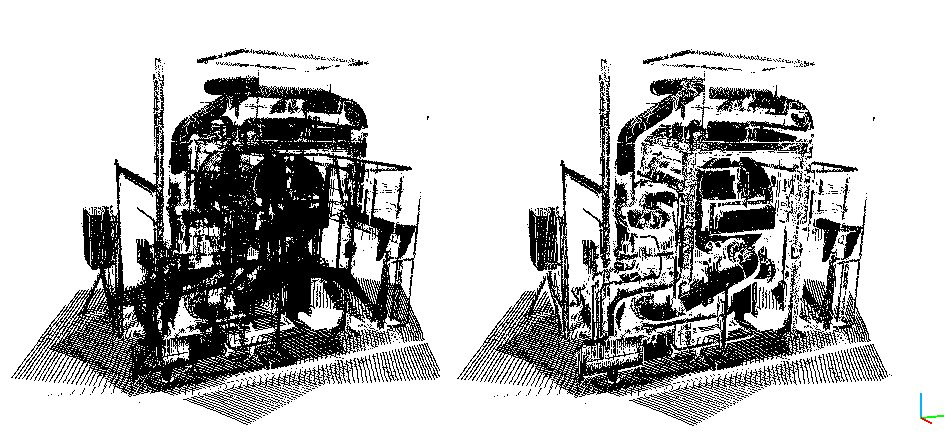
\includegraphics[width=0.5\textwidth]{Partie3_Fonctions/HPRExample.jpg}
\caption{\label{fig:PCVExample}Nuage de point complet (en haut) et nuage de point filtr� avec la technique "HPR" (en bas)}
\end{center}
\end{figure}

\par
La notion de visibilit� pour les points d'un nuage est relativement complexe � estimer.
En effet il est tr�s peu probable qu'un point soit r�ellement masqu� par
d'autres points dans un nuage, puisque cel� n�cessiterait un alignement parfait entre paires
de points ou une densit� du nuage telle que les points soient quasiment en contact. Cette fonction
approxime donc la notion de visibilit� via un calcul d'enveloppe convexe. Elle se base sur l'article
\emph{Direct Visibility of Point Sets} de Katz, Tal et Basri, SIGGRAPH 2007.
\\
\par
Pour calculer les occlusions par HPR, il est n�cessaire que le contexte graphique du nuage soit en
projection perspective (cf. section \ref{subsection:centeredPerspective}). Si ce n'est pas le cas,
un message d'erreur pr�vient l'utilisateur lui demandant d'activer la projection perspective\index{projection!pour visualisation}.
L'utilisateur doit ensuite choisir le niveau d'octree utilis� par la fonction (figure \ref{fig:HPRLevelChoice}).
Le niveau d'octree\index{octree} permet d'acc�lerer le calcul de l'enveloppe convexe (structure assez lourde)
en r�duisant le nombre de points utilis�s (par sous-�chantillonnage). Plus le niveau est �lev�, et plus
le calcul d'occlusion sera fin, mais plus le traitement sera long.
\\

\begin{figure}[!htb]
\begin{center}
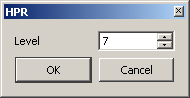
\includegraphics[width=0.3\textwidth]{Partie3_Fonctions/HPRLevelChoice}
\caption{\label{fig:HPRLevelChoice}Interface de choix de niveau d'octree}
\end{center}
\end{figure}

\par
Une fois le filtrage effectu�, celui-ci n'est valide que pour la position de cam�ra courante (et des positions tr�s
proches dans une certaine mensure). Il faut relancer l'outil pour mettre � jour le filtrage selon tout nouveau point
de vue.\\
\par
\textcolor[rgb]{1.00,0.00,0.00}{Attention, les points cach�s par cette m�thodes ne peuvent pas �tre r�-affich�s
via une m�thode ad-hoc (pour l'instant). Il faut en attendant utiliser un artifice : activer l'outil de segmentation
manuelle sur le nuage (l'ic�ne des "ciseaux" - section~\ref{subsection:graphicalSegmentation}) qui r�initialise
l'information de visibilit� par point) puis quitter ce mode.}
